\subsection{\ab{Simulations using GR signals in Gaussian noise}} \label{ssec:gr_signal}

\ab{We demonstrate our method using synthetic-signal injections describing GWs
from BBHs in GR. We employ coloured Gaussian noise with PSDs expected for LIGO and
Virgo detectors at design sensitivities~\cite{}. \comment{AB: Please cite which PSD you used.}
For the mock BBH signals, we choose parameters similar to two specific GW events, GW150914~\cite{} and
GW190521~\cite{}. We list them in Table~\ref{tab:injection_values}.
These two binary systems are representative of the kind of systems for which
the QNM measurement is most suitable, notably high-mass BBH events which are loud enough that the
pre- and post-merger SNRs return reliable parameter-estimation results.}

%%%%%%%%%%%%%%%%%%%%%%%%%%%%%%%%%%%%%%%%%%%%%%%%%%%%%%%%%%%%%%%
% Table for Injections
%%%%%%%%%%%%%%%%%%%%%%%%%%%%%%%%%%%%%%%%%%%%%%%%%%%%%%%%%%%%%%%
\begin{table}[h!]
\begin{center}
\begin{tabular}{ |c|c|c|c|c|c| }
 \hline
 Event & $m_{\rm 1,det} (\Mo)$ &  $m_{\rm 2,det} (\Mo)$ & $\chi_{1}$ & $\chi_{2}$ & SNR \\
 \hline
 GW150914-like & 39 & 31 & 0.0 & 0.0 & 25 \\
 GW190521-like & 150 & 120 & 0.02 & -0.39 & 14 \\
 SXS:BBH:0166 & 72 & 12  & 0.0 & 0.0 & 75 \\
 \hline
\end{tabular}
\caption{\ab{Parameters of the synthetic-signal injections}, chosen to be similar to the actual GW events indicated in the first column. The parameters
$(m_{\rm 1,det},m_{\rm 2,det})$ are the detector-frame masses of the primary and secondary BHs, respectively. \comment{AB: I would suggest to give in the Table also the SNR in the pre- and post-merger stages. The third row is completely ignored in the caption's explanations.}}
\label{tab:injection_values}
\end{center}
\end{table}
%%%%%%%%%%%%%%%%%%%%%%%%%%%%%%%%%%%%%%%%%%%%%%%%%%%%%%%%%%%%%%%
%%%%%%%%%%%%%%%%%%%%%%%%%%%%%%%%%%%%%%%%%%%%%%%%%%%%%%%%%%%%%%%

\comment{AB: Nothing is said in the text and the caption of the Table about the third mock signal in the Table!}

%%%%%%%%%%%%%%%%%%%%%%%%%%%%%%%%%%%%%%%%%%%%%%%%%%%%%%%%%%%%%%%
% Simulated siganl: GR
%%%%%%%%%%%%%%%%%%%%%%%%%%%%%%%%%%%%%%%%%%%%%%%%%%%%%%%%%%%%%%%
\begin{figure*}[hbt]
\begin{center}
        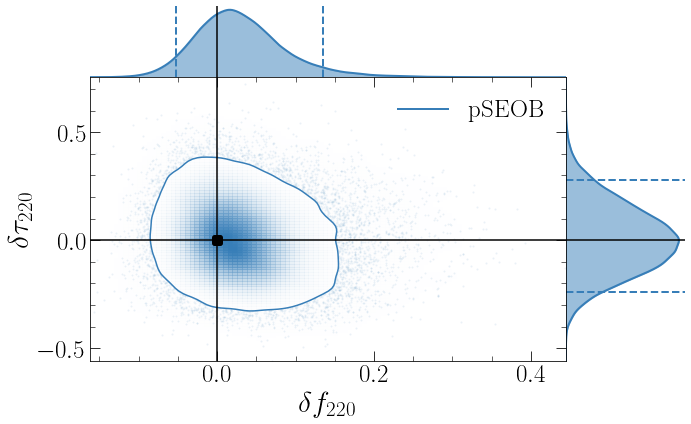
\includegraphics[width=0.5\textwidth]{figures/GW150914_simulated_signal_0p0_deltaf220_deltatau220.png}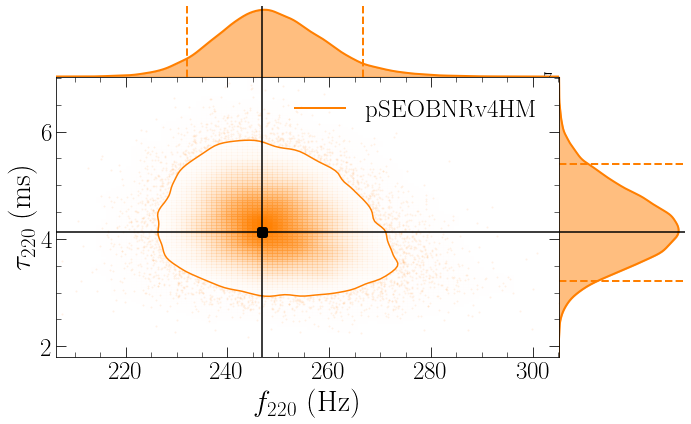
\includegraphics[width=0.5\textwidth]{figures/GW150914_simulated_signal_0p0_f220_tau220.png}
        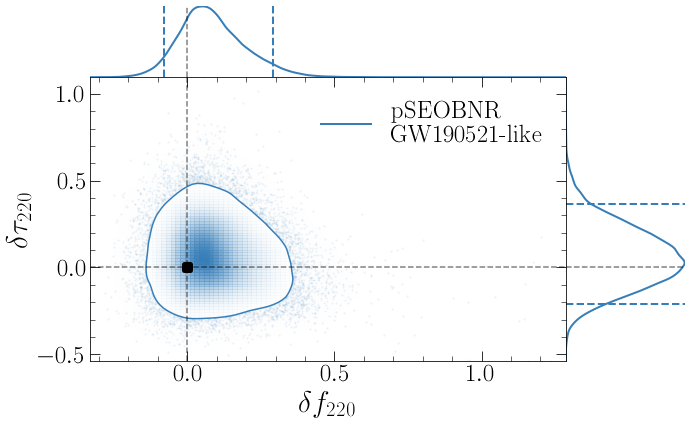
\includegraphics[width=0.5\textwidth]{figures/GW190521_simulated_signal_0p0_deltaf220_deltatau220.png}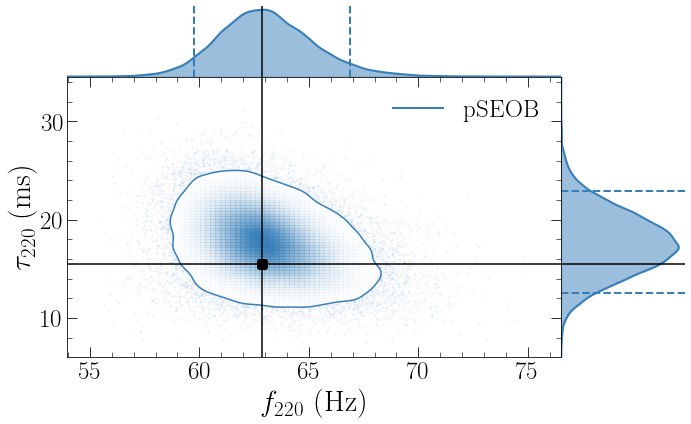
\includegraphics[width=0.5\textwidth]{figures/GW190521_simulated_signal_0p0_f220_tau220.png}
        \caption{\textcolor{red}{FINAL RESULT} Posterior probability distribution on the fractional deviations in the frequency and damping time of the $(2,2)$ QNM, $(\df{220},\dtau{220})$ (left panels) and the reconstructed quantities, $(\fngr{220}, \taungr{220})$ (right panels) for GR injections with initial parameters similar to GW150914 (top panels) and GW190521 (bottom panels) (Table~\ref{tab:injection_values}). The 2D contour marks the 90\% credible region, while the dashed lines on the 1D marginalized distributions mark the 90\% credible levels. The black vertical and horizontal lines mark the injection values. \comment{AB: Please indicate on the figures: GW150914-like and GW190521-like.} \comment{AB: Please be consistent and use the label pSEOBNR, as in the text, instead of pSEOB.}}
        \label{fig:simulated_signal_GR}
\end{center}
\end{figure*}
%%%%%%%%%%%%%%%%%%%%%%%%%%%%%%%%%%%%%%%%%%%%%%%%%%%%%%%%%%%%%%%
%%%%%%%%%%%%%%%%%%%%%%%%%%%%%%%%%%%%%%%%%%%%%%%%%%%%%%%%%%%%%%%

\ab{To avoid possible systematic biases in our parameter-estimation analysis
due to error in waveform modeling,} we use the GR version of the same waveform,
$\SEOB$ (without allowing for deviations in the QNM parameters) to
simulate our GW signal. And to avoid systematic biases due to noise,
we use an averaged (zero-noise) realization of the noise. A detailed
study on noise systematics for one of the GW events is presented in
Appendix~\ref{sec:noise_systematics}. \comment{AB: This reference to the Appendix is out of context.
Why should the reader appreciate at this stage of the paper, where we have not yet
discussed results with real data, what is in the Appendix?} As in the case of the actual
detections, we consider a two-detector LIGO network at
Hanford and Livingston, having identical PSDs. The distance to the two
\ab{synthetic} events is rescaled such that the SNR in the detector network
is the same as the actual events (i.e., 24 for GW150914 and 14
for GW190521). Since mearly--equal-mass binaries like GW150914 and
GW190521 observed at moderately high SNRs are not expected to have a
loud ringdown signal, we restrict ourselves to estimating the
frequency and damping time of \ab{only one QNM} $(\ell m) = (2,2)$, i.e.,
$\{\df{220},\dtau{220}\}$, while fixing the other QNM frequencies to
their GR values.

We find, as one might expect, that the posterior distribution on the
parameters describing fractional deviations in the frequency and
damping time are consistent with zero (left panels of
Fig.~\ref{fig:simulated_signal_GR}). One can then convert these
fractional quantities into absolute quantities using the relations
given in Eqs.~\ref{eq:nongr_freqs_a} and ~\ref{eq:nongr_freqs_b}, and
construct posterior distributions on these effective quantities,
$(\fngr{220}, \taungr{220})$ (right panels of
Fig.~\ref{fig:simulated_signal_GR}). In each of these cases, the recovered
\ab{2D} posterior{\ab{s} are consistent with the GR predictions
(black \sout{solid lines} \ab{dot}). \comment{AB: please be precise in referring
to 1D and 2D posteriors when discussing the figures.}}


\subsection{\ab{Simulations using non-GR signals in Gaussian noise}} \label{ssec:ngr_signal}


To demonstrate the robustness of the method in detecting possible
deviations \sout{of the underlying GW signal from predictions of} \ab{from GR},
we inject \sout{simulated} \ab{synthetic} GW signals which are identical to
the corresponding GR prediction up to merger, and differ in their post-merger
description. We again choose \sout{systems with initial-}binary-parameters
similar to GW150914 and GW190521 (as given in Table XXX), but
\sout{we attach a phenomenological post-merger signal described by deviation parameters}
\ab{set} $\df{220} = \dtau{220} = 0.5$ \comment{AG: deviations=0.1 runs are ongoing and almost
  done. AB: I would show results that include the $10\%$ case, which is more realistic,
based on QNM predictions in theories of gravity alternative to GR.}.
In other words, we assume that the frequency and damping time
of our non-GR signal is 1.5 times the corresponding GR prediction,
although the pre-merger signal is identical to GR. \ab{In Fig.~\ref{fig:nongr_waveform}
we show ...}  \comment{AB: Not clear to me what the next sentence says. Coudl
you just clearly refer to thePlease introduce the injected signal and the template, which is used
to recover it, and simply say that they belong to the same waweform model.}
We also avoid waveform \sout{and noise} systematic biases by choosing
a configuration identical to the simulations described in Sec.\ref{ssec:gr_signal}. \ab{We
summarize the results of the Bayesian analysis in Fig.~\ref{fig:simulated_signal_nonGR} where we
show the posterior probability distributions for $(\df{220}, \dtau{220})$, or equivalently
$(\fngr{220}, \taungr{220})$. We find that they are consistent with the corresponding
values of the injection parameters, indicated by the black solid lines.} \comment{AB: Please be more quantitative when
explaining the results in the figure. Which black lines are you referring to? In the main 2-D figure the injected signal
is a point not a line. I think you are referring to the 1D posteriors, but it needs to be explained.}

We additionally investigate the effects of erroneously assuming that
\sout{an underlying modified} \ab{a non-GR} signal can be well-described
\ab{by a GR one}. We do this by estimating the parameters of our \ab{non-GR}
signals using the GR waveform model $\SEOB$ instead of the parameterized
$\pSEOB$. \comment{AB: Not clear what the next senetnce wants to say.}
In such cases, we run the risk of biased parameter estimates due to an
incomplete understanding of the underlying signal. The resulting
posterior probability distributions are shown in the right panels of
Fig.~\ref{fig:simulated_signal_nonGR} by the \ab{red (GW150914-like) and blue
(GW190521-like) curves.} The results are interesting and distinctly
different for the two events. For the GW150914-like \comment{AB: I would avoid using
``modified'' GR, but istsead non-GR.} \ab{non-GR} signal, the measurements of $(\fgr{220}, \taugr{220})$
(see top right panel in Fig.~\ref{fig:simulated_signal_nonGR}) are consistent
with the $(\fgr{220}, \taugr{220})$ measurements for a signal with no
deviations from GR (see top right panel in Fig.~\ref{fig:simulated_signal_GR}). In other
words, if the actual signal had deviations \ab{from GR} as large as the $50\%$ \sout{of
the GR prediction}, the analysis with \ab{the GR signal} $\SEOB$ would likely have
reported \emph{no} deviation from the GR prediction. However in the
case of the GW190521-like \ab{non-GR} signal, a simple GR analysis of
the non-GR signal would have yielded measurements distinctly
different from either of the two parameterized estimates: with and
without deviations. \comment{AB: Not clear to me the next sentence. We are working
in Gaussian noise, so why are you referring to the noise as the culprit or the
source of difference?} The fact that the GW190521-like signal has a much
lower SNR than GW150914-like signal might be a possible reason for the
measurement of the final quantities to be more susceptible to noise. A
more detailed comparison of the other parameters, like the masses and
spins, between an $\pSEOB$ and an $\SEOB$ measurement of a modified GR
signal is shown in Fig.~\ref{fig:gr_ngr_comparison}. \comment{AB: Please
comment the figures. What are the main results? What do we deduce?}

%%%%%%%%%%%%%%%%%%%%%%%%%%%%%%%%%%%%%%%%%%%%%%%%%%%%%%%%%%%%%%%
%%%%%%%%%%%%%%%%%%%%%%%%%%%%%%%%%%%%%%%%%%%%%%%%%%%%%%%%%%%%%%%
\begin{figure}
        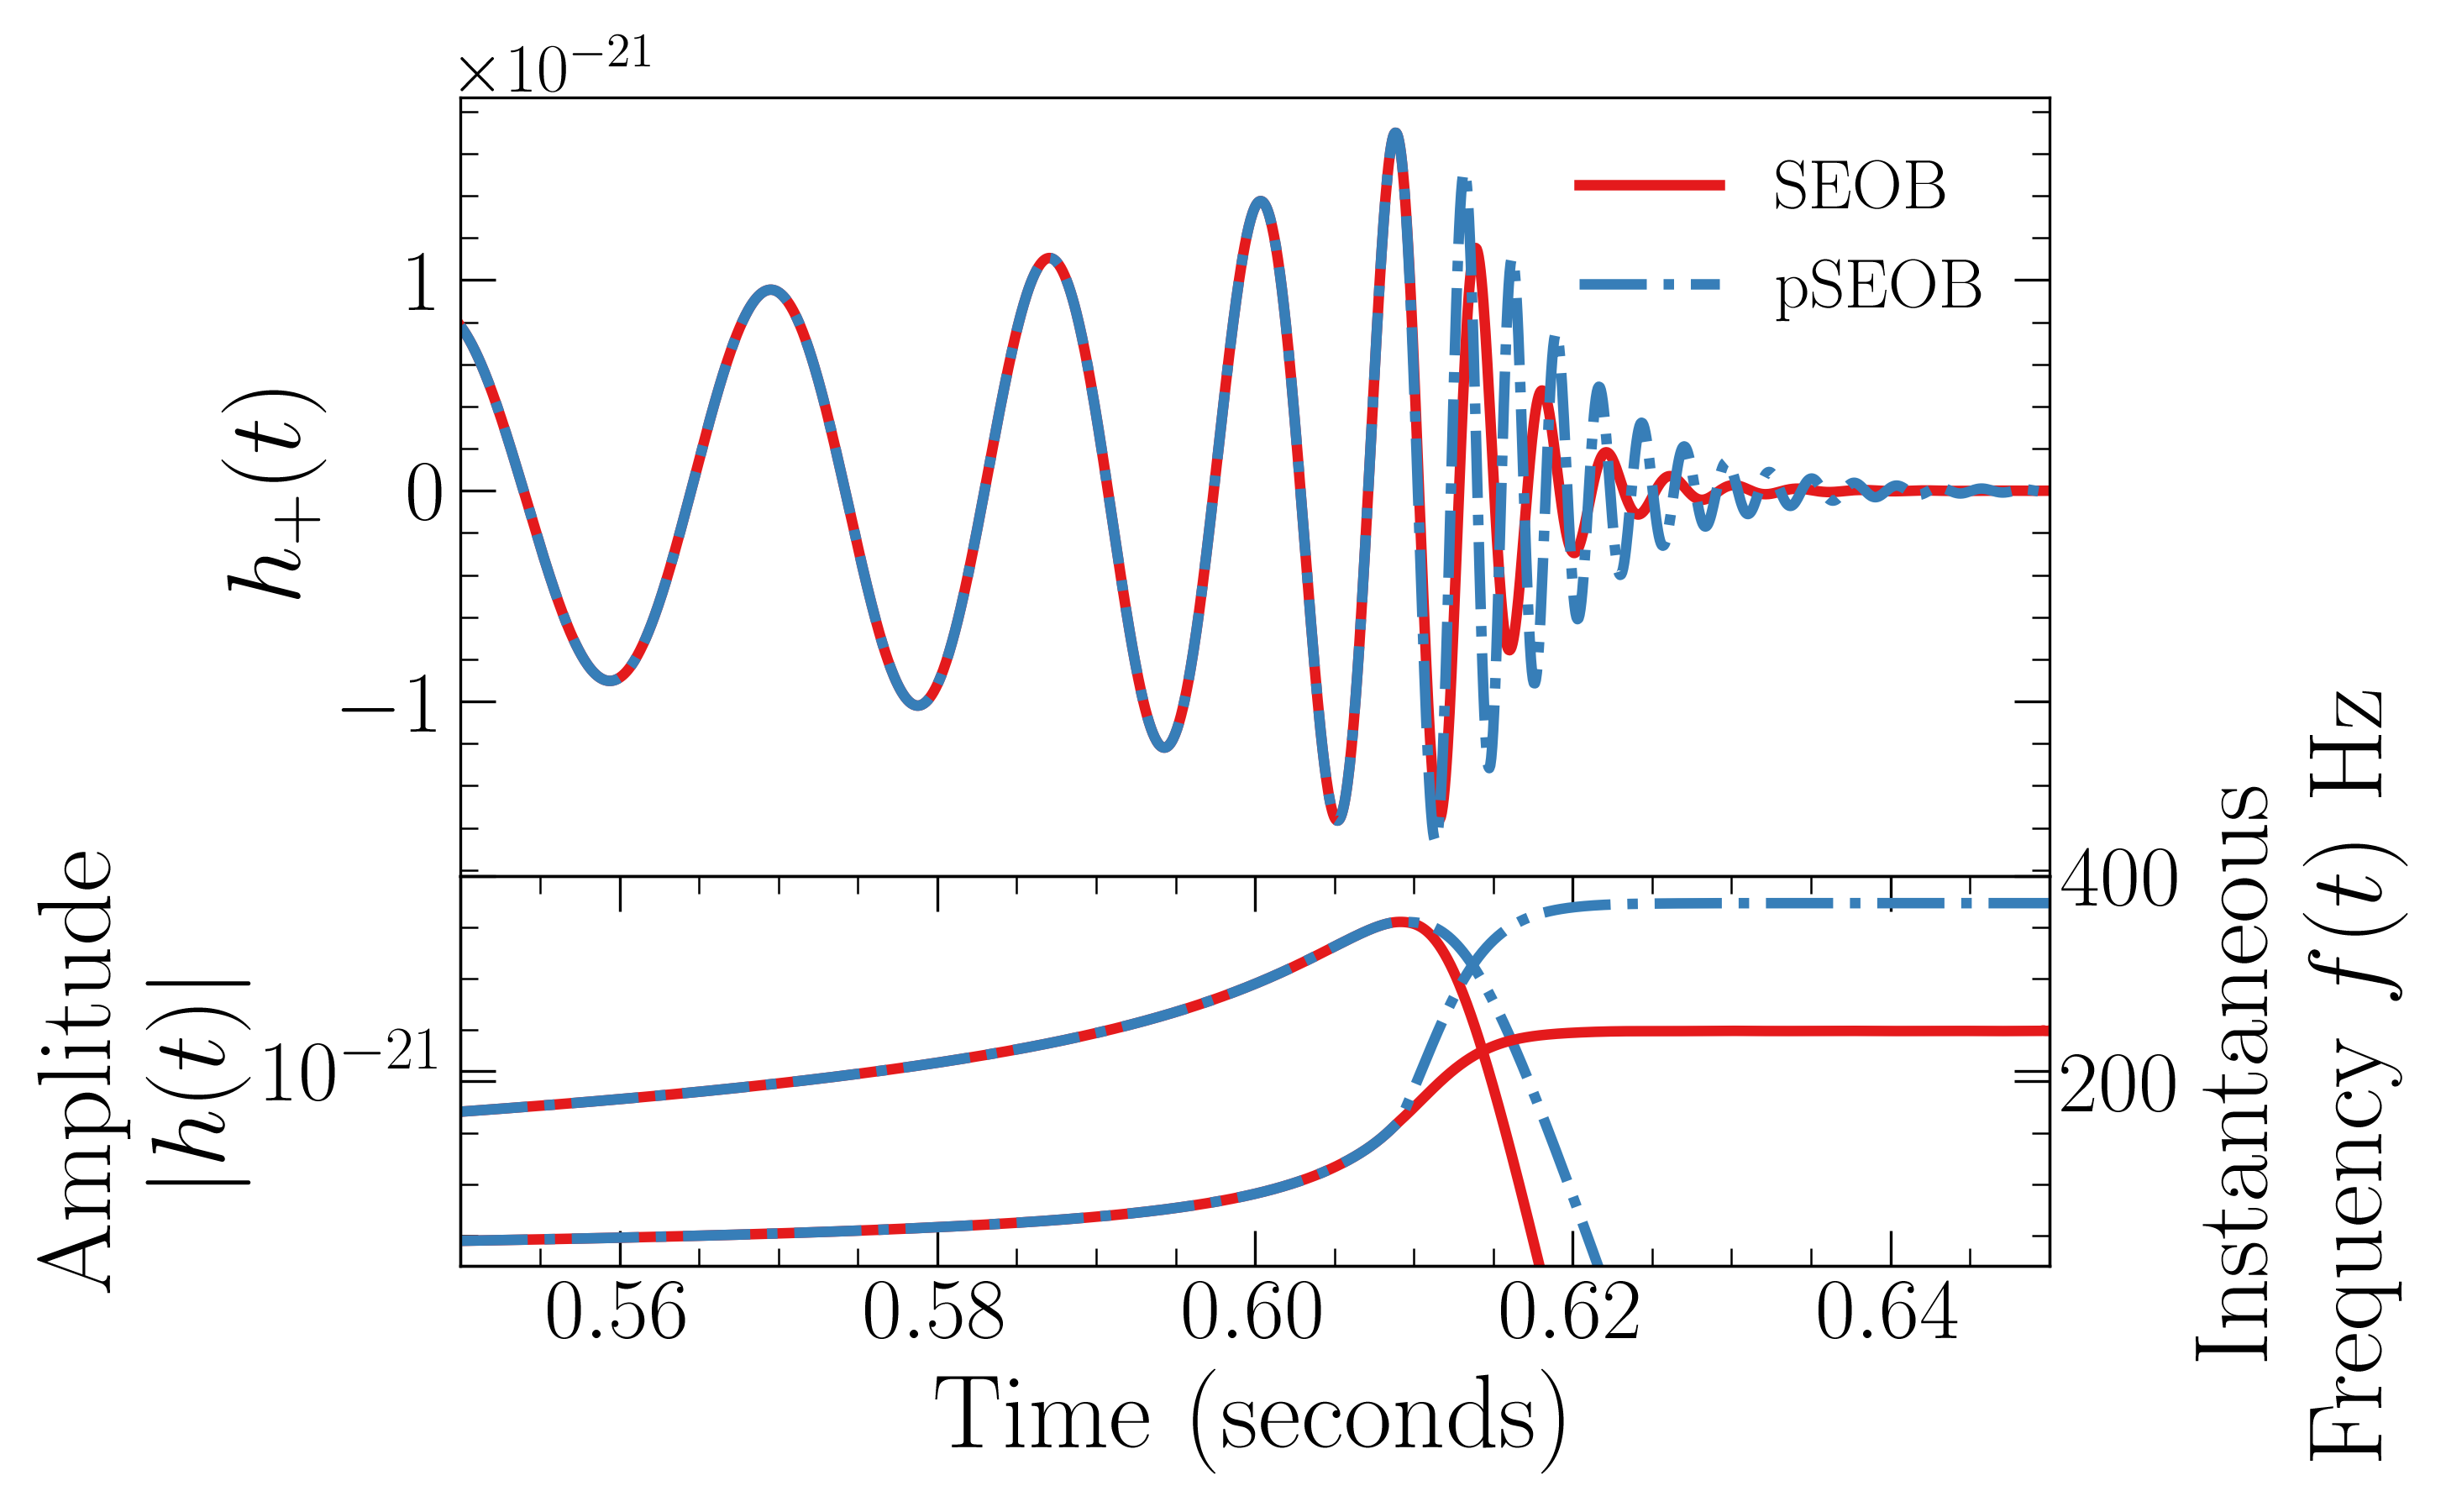
\includegraphics[width=0.5\textwidth]{figures/modGR_waveforms_amplitudephase.png}
        \caption{\textcolor{red}{FINAL RESULT} Top panel: The `+'--polarization of the gravitational waveform $h_+(t)$ from a GW150914-like event where the post-merger is described by GR \sout{(solid orange lines)} (i.e., $\df{220} = \dtau{220} = 0$), and where the merger-ringdown is modified \sout{(dashed grey lines)} (i.e., $\df{220} = \dtau{220} = 0.5$). Bottom panel: Comparison of the evolution of the amplitude (left) and instantaneous frequency (right) for the GR and \sout{modified} \ab{non-GR} signal. \comment{AB: Please remove ``Amplitudes'' and ``Instantaneous Frequency'' from the $y$-axis labels, but instead provide explanations in the caption, and use only $f(t)$ as label.}}
        \label{fig:nongr_waveform}
\end{figure}
%%%%%%%%%%%%%%%%%%%%%%%%%%%%%%%%%%%%%%%%%%%%%%%%%%%%%%%%%%%%%%%
%%%%%%%%%%%%%%%%%%%%%%%%%%%%%%%%%%%%%%%%%%%%%%%%%%%%%%%%%%%%%%%

%%%%%%%%%%%%%%%%%%%%%%%%%%%%%%%%%%%%%%%%%%%%%%%%%%%%%%%%%%%%%%%
% Simulated siganl: non-GR
%%%%%%%%%%%%%%%%%%%%%%%%%%%%%%%%%%%%%%%%%%%%%%%%%%%%%%%%%%%%%%%
\begin{figure*}%[h!]
\begin{center}
        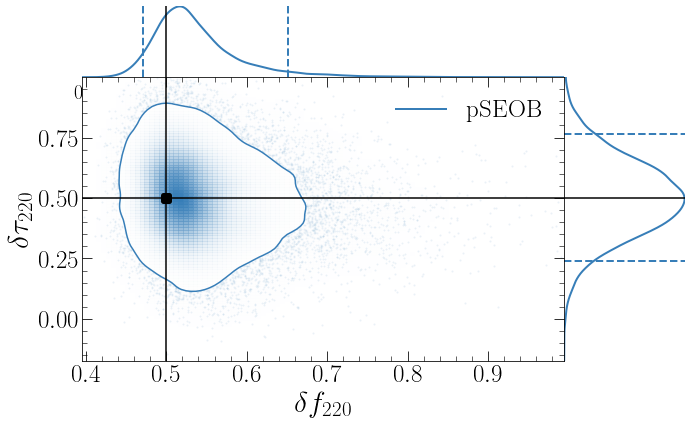
\includegraphics[width=0.5\textwidth]{figures/GW150914_simulated_signal_0p5_deltaf220_deltatau220.png}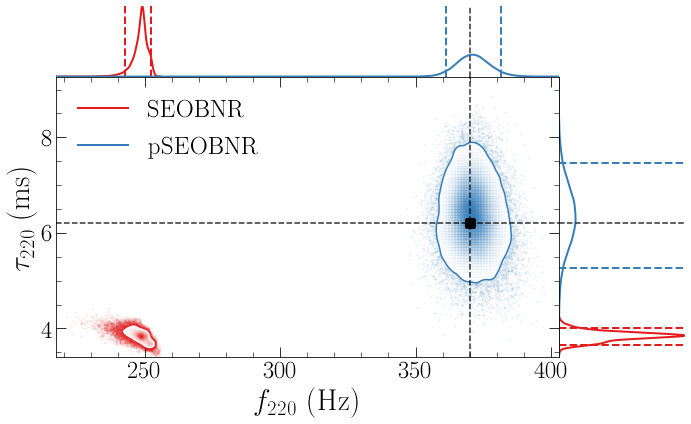
\includegraphics[width=0.5\textwidth]{figures/GW150914_simulated_signal_0p5_gr_ngr_fngrtaungr.png}
        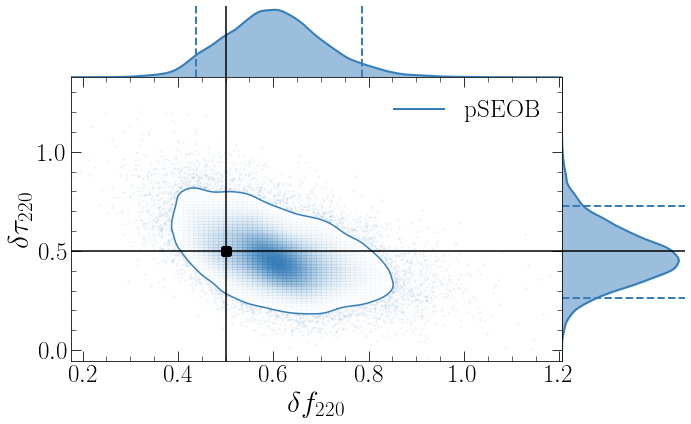
\includegraphics[width=0.5\textwidth]{figures/GW190521_simulated_signal_0p5_deltaf220_deltatau220.png}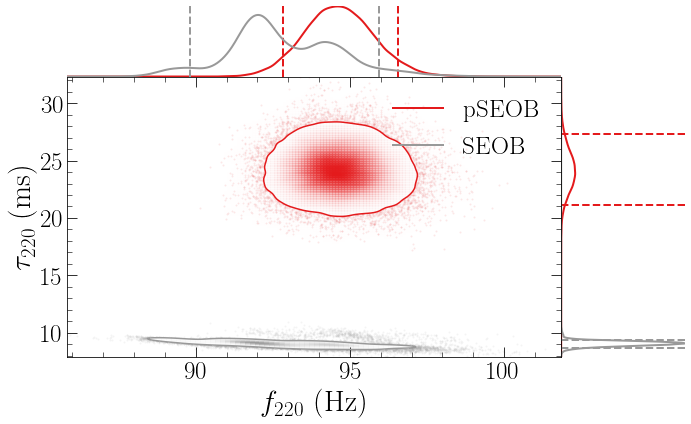
\includegraphics[width=0.5\textwidth]{figures/GW190521_simulated_signal_0p5_gr_ngr_fngrtaungr.png}
        \caption{\textcolor{red}{FINAL RESULT} Posterior probability distribution on the fractional deviations in the frequency and damping time of the $(2,2)$ QNM, $(\df{220},\dtau{220})$ (left panels) and the reconstructed quantities, $(\fngr{220}, \taungr{220})$ (right panels) for \sout{modGR} \ab{non-GR} injections with \sout{initia}l parameters \sout{similar to} \ab{of GW150914-like} (top panels) and \ab{GW190521-like} (bottom panels) \ab{as given in Table~\ref{tab:injection_values}.} The \sout{underlying} \ab{non-GR} signal has a deviation, $\df{220} = \dtau{220} = XX$. The 2D contour marks the 90\% credible region, while the dashed lines on the 1D marginalized distributions mark the 90\% credible levels. The black vertical and horizontal lines mark the injection values. In the right panels, we additionally show measurements using a GR ($\SEOB$) waveform, for the
GW150914-like \sout{(grey)} \ab{(upper panel)} and GW190521-like \sout{(pink)} \ab{(lower panel) injections}. The measurements \ab{with $\SEOB$ waveforms} are visibly biased. \comment{AB: please
switch the red and blue colors. The blue colors should always refer to the same waveform model, which is shown in the left panels, otherwise it is very confusing to understand those plots. Please indicate on the figures: GW150914-like and GW190521-like.}}
        \label{fig:simulated_signal_nonGR}
\end{center}
\end{figure*}
%%%%%%%%%%%%%%%%%%%%%%%%%%%%%%%%%%%%%%%%%%%%%%%%%%%%%%%%%%%%%%%
%%%%%%%%%%%%%%%%%%%%%%%%%%%%%%%%%%%%%%%%%%%%%%%%%%%%%%%%%%%%%%%

%%%%%%%%%%%%%%%%%%%%%%%%%%%%%%%%%%%%%%%%%%%%%%%%%%%%%%%%%%%%%%%
% modified GR signal: GR vs nonGR recovery comparison
%%%%%%%%%%%%%%%%%%%%%%%%%%%%%%%%%%%%%%%%%%%%%%%%%%%%%%%%%%%%%%%
\begin{figure*}%[h!]
        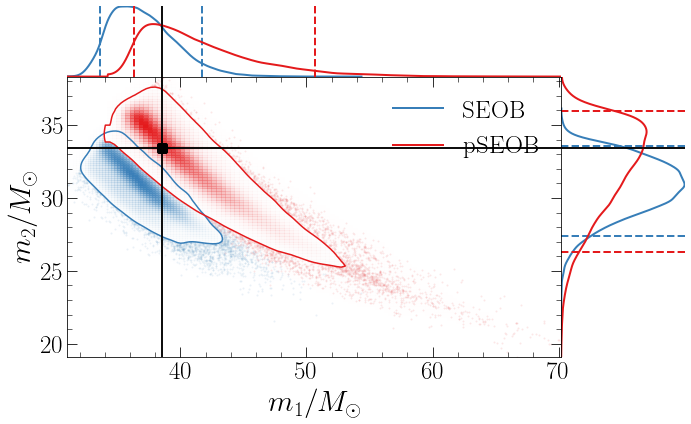
\includegraphics[width=0.5\textwidth]{figures/GW150914_simulated_signal_0p5_gr_ngr_m1m2.png}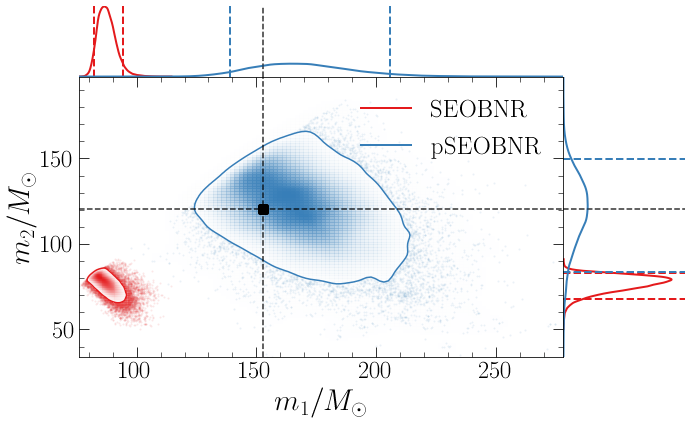
\includegraphics[width=0.5\textwidth]{figures/GW190521_simulated_signal_0p5_gr_ngr_m1m2.png}
        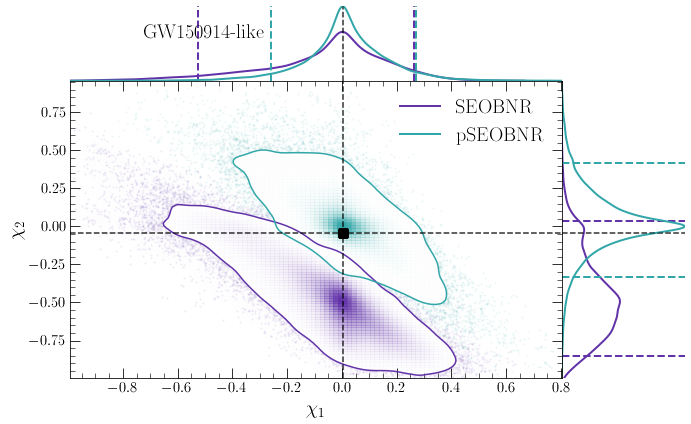
\includegraphics[width=0.5\textwidth]{figures/GW150914_simulated_signal_0p5_gr_ngr_a1za2z.png}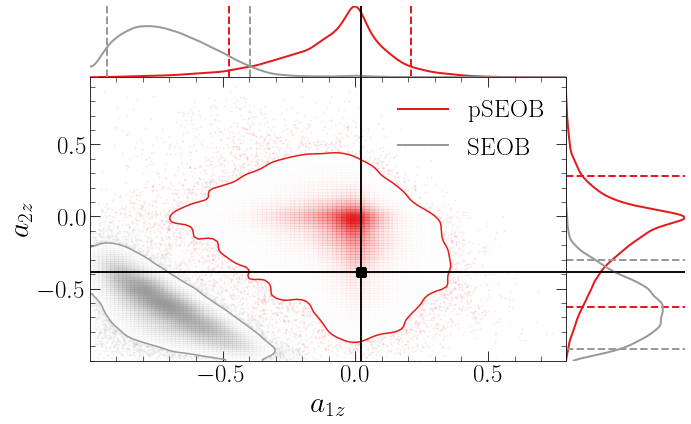
\includegraphics[width=0.5\textwidth]{figures/GW190521_simulated_signal_0p5_gr_ngr_a1za2z.png}
        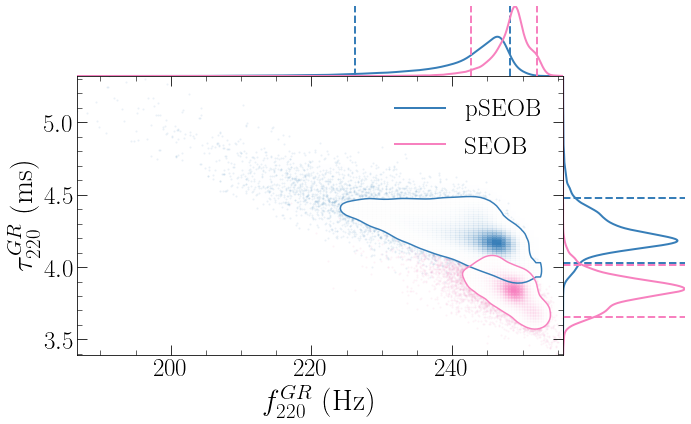
\includegraphics[width=0.5\textwidth]{figures/GW150914_simulated_signal_0p5_gr_ngr_fgrtaugr.png}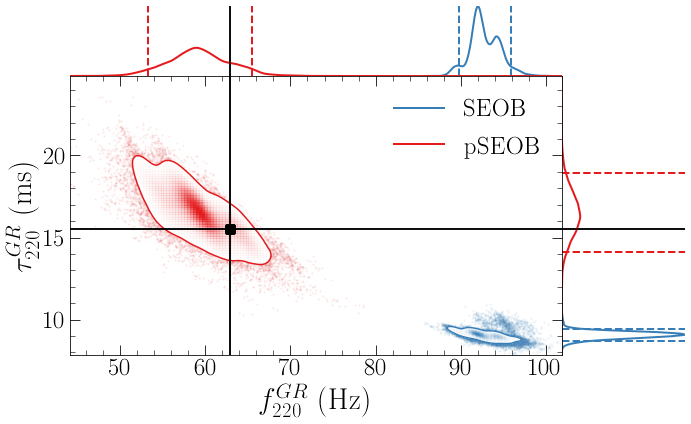
\includegraphics[width=0.5\textwidth]{figures/GW190521_simulated_signal_0p5_gr_ngr_fgrtaugr.png}
        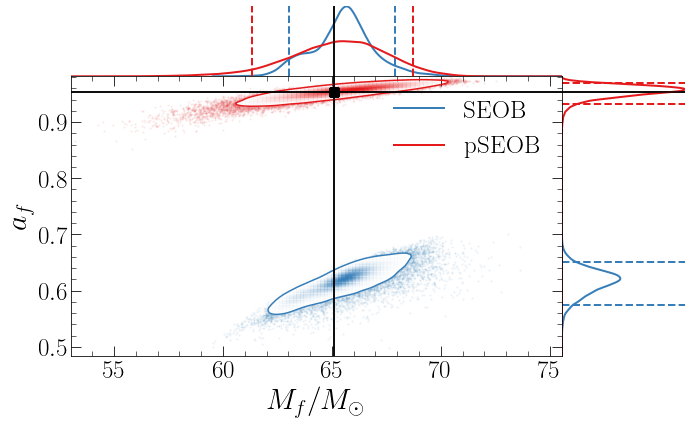
\includegraphics[width=0.5\textwidth]{figures/GW150914_simulated_signal_0p5_gr_ngr_Mfaf.png}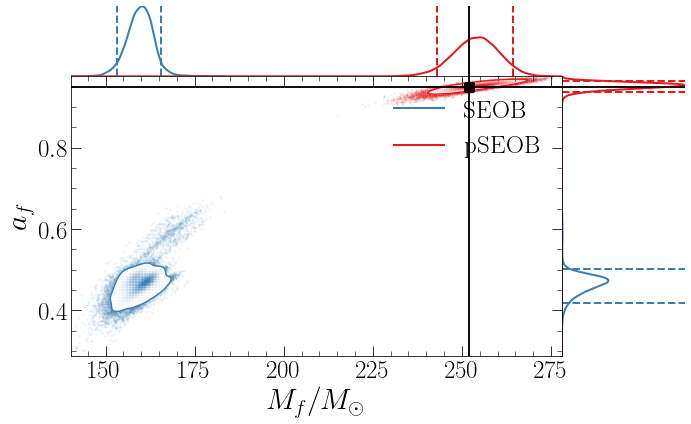
\includegraphics[width=0.5\textwidth]{figures/GW190521_simulated_signal_0p5_gr_ngr_Mfaf.png}
        \caption{\textcolor{red}{FINAL RESULT} Comparison of \sout{the recovered} \ab{binary's} parameters when \sout{the underlying signal is assumed to be a GR signal or a modified GR signal} \ab{a non-GR signal ($\pSEOB$) is injected and recovered with a GR ($\SEOB$) or a non-GR ($\pSEOB$) waveform model}. \sout{In both cases, the actual underlying signal is a modified GR signal with parameters similar to} \ab{The left (right) panels refer to
a GW150914-like (GW190521- like) injected signal (see Table~\ref{tab:injection_values}) with QNM deviation parameters of $\df{220} = \dtau{220} = 0.5$.} \sout{For the GW150914 (GW190521) contours, the $SEOB$ and $pSEOB$ recoveries are indicated by blue (red) and pink (grey) curves respectively.} The panels (from top to bottom) show the recoveries in (detector-frame) \sout{initial} masses (first row), \sout{z-components of dimensionless initial} \ab(dimensionless) spins (second row), GR predictions of frequency and damping time (third row) and the remnant mass and spin predictions ($M_f$, $a_f$) from the frequency and damping time
(obtained by inverting the Berti fits). \comment{AB: I would write those details about the ``Berti's fits, etc.'' in the text, not in the caption. Also please specify if the remnant mass is the detector-frame mass. Please
switch the red and blue colors. The blue colors should always refer to the same waveform model, i.e., $\pSEOB$. Please indicate on the figures: GW150914-like and GW190521-like.}}
        \label{fig:gr_ngr_comparison}
\end{figure*}
%%%%%%%%%%%%%%%%%%%%%%%%%%%%%%%%%%%%%%%%%%%%%%%%%%%%%%%%%%%%%%%
%%%%%%%%%%%%%%%%%%%%%%%%%%%%%%%%%%%%%%%%%%%%%%%%%%%%%%%%%%%%%%%


\subsection{Test of the no-hair conjecture}\label{ssec:nohairtheorem}

Finally, we provide a simple demonstration of a test of the no-hair
theorem using our model. As described in the introduction, any test of
the no-hair theorem of BHs would need to involve independent
measurements of (at least) two different QNMs.

\ab{Here, we} use a \sout{simulated} NR GW signal from the SXS catalog~\cite{}
corresponding to a non-spinning BBH with mass-ratio $q=6$ (SXS:BBH:0166),
\sout{rescaled to a} total mass $M=84 \Mo$ (see Table~\ref{tab:injection_values}).
We choose an asymmetric system to increase the SNR in the higher modes.
We also \sout{rescale} \ab{choose} the distance and orientation of the binary
such that the total SNR \sout{of the signal} in \sout{a} \ab{the} network of
the three detectors, LIGO Hanford, Livingston and
Virgo, is 75. Based on the LIGO-Virgo observations during O3a, such
asymmetric and loud signals are no longer just a theoretical
prediction, but quite plausible at design sensitivities. Using this
signal, we attempt to measure \ab{both} the \sout{QNM frequencies} $(2,\pm 2)$ and
$(3,\pm 3)$ \sout{modes} \ab{QNMs} \sout{together}. \ab{We summarize
our results in Fig.~\ref{fig:nohair_sxs}. For this injected signal the SNR in
other sub-dominant modes is too low to be able to measure them.} \sout{less for us to estimate them reliably.}

The fractional deviations in the estimates of the damping time and
frequency of either mode is expected to be consistent with 0, as we
indeed find in the left panel of
Fig.~\ref{fig:nohair_sxs}. Consequently we find that the reconstructed
quantities $(\fngr{220}, \taungr{220})$ and $(\fngr{330},
\taungr{330})$ are also consistent with the corresponding predictions
for a BBH merger in GR. As a consequence, the information from these
two independent measures correspond to a unique remnant object, which
is completely described by its mass and spin angular momentum
\abhi{have the mf-af plot as well as a third panel to show
  consistency}. For most of the events observed so far, the power in
the $(3,\pm 3)$ has not been sufficient to measure it along with the
$(2,\pm 2)$, or in fact, in its place. However, it might also be
possible to combine information from multiple observation\sout{, as is
likely} over the coming few years \sout{of GW astronomy with the LIGO-Virgo
detectors,} to obtain meaningful constraints on the $(3,\pm 3)$ and
other sub-dominant QNMs~\cite{}.

%%%%%%%%%%%%%%%%%%%%%%%%%%%%%%%%%%%%%%%%%%%%%%%%%%%%%%%%%%%%%%%

%%%%%%%%%%%%%%%%%%%%%%%%%%%%%%%%%%%%%%%%%%%%%%%%%%%%%%%%%%%%%%%
\begin{figure}
        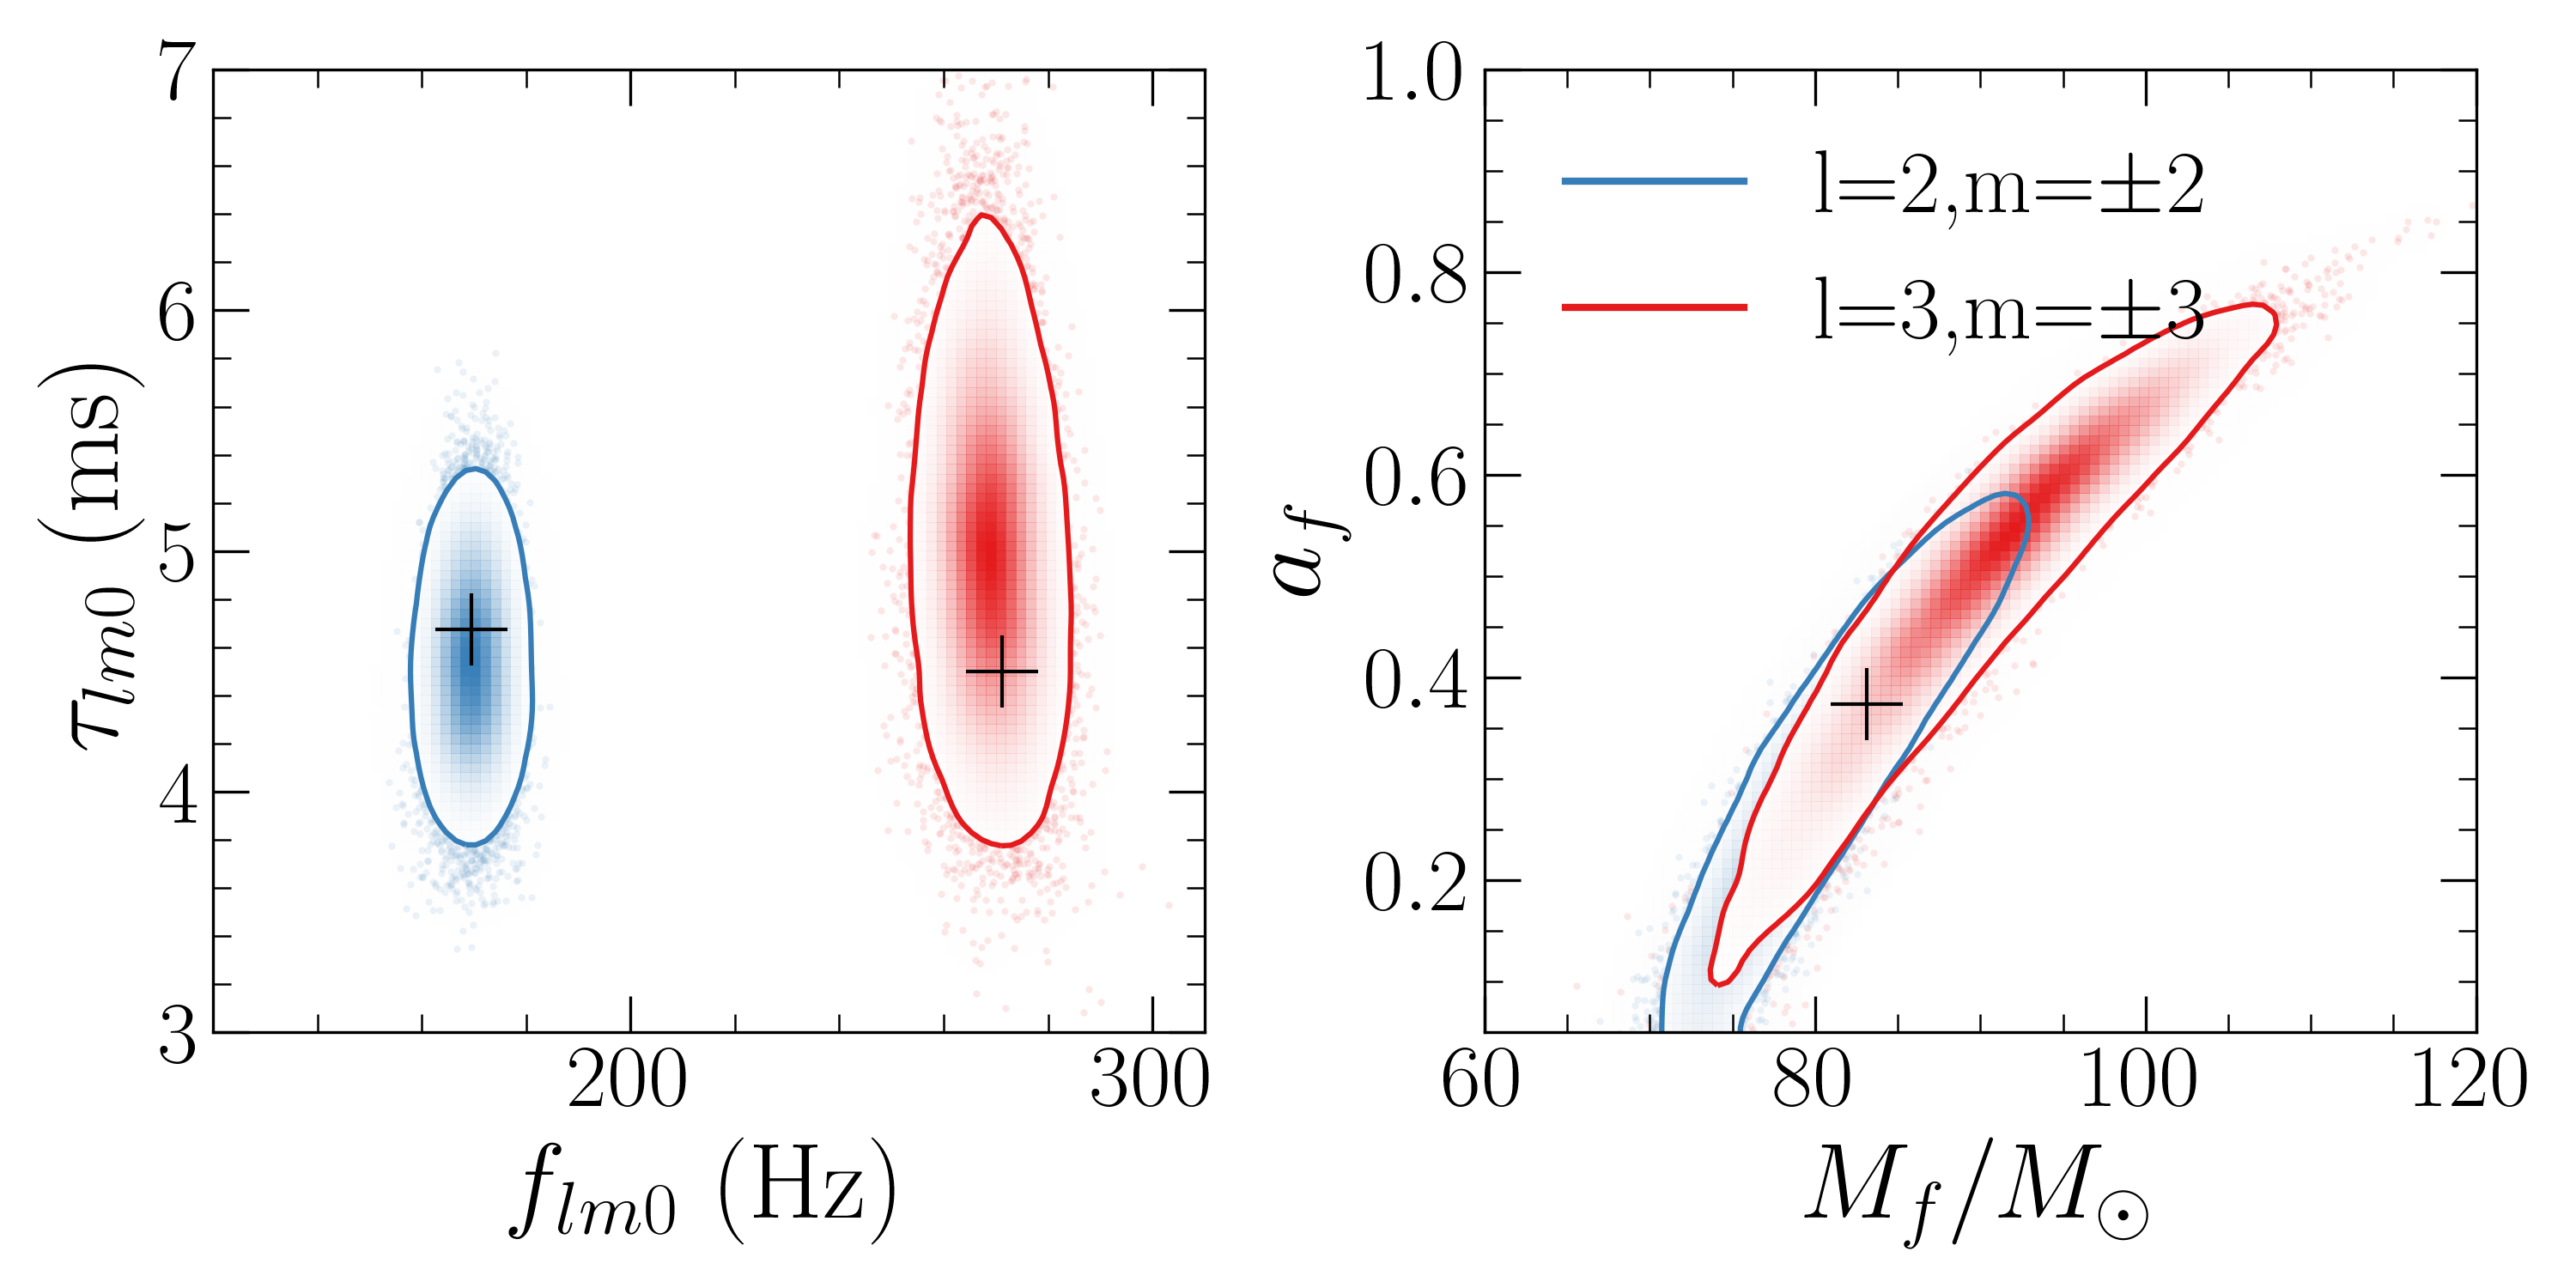
\includegraphics[width=0.5\textwidth]{figures/nohair_sxs_0166.png}
        \caption{\textcolor{red}{PRELIMINARY} Posterior probability distribution on the fractional deviations (left panel) and the reconstructed (right panel) frequency and damping time of the $(2,\pm 2)$ (blue curves) and $(3,\pm 3)$ (red curves) \ab{QNM,} respectively, \sout{for a numerical relativity signal corresponding to a BBH merger of} \ab{when a NR signal with parameters} $q=6$,  $M=84 \Mo$ and SNR $=75$ \ab{is injected in Gaussian noise and recovered with the $\pSEOB$ waveform model}. The plus signs mark the GR predictions.}
        \label{fig:nohair_sxs}
\end{figure}
%%%%%%%%%%%%%%%%%%%%%%%%%%%%%%%%%%%%%%%%%%%%%%%%%%%%%%%%%%%%%%%
%%%%%%%%%%%%%%%%%%%%%%%%%%%%%%%%%%%%%%%%%%%%%%%%%%%%%%%%%%%%%%%
